\chapter{Visualization}
We first begin our analysis by looking at cumulative returns, an essential part of time series analysis. Unlike daily or periodic returns, which can be volatile, cumulative returns smooth out fluctuations and show the overall trends of a time series. They also help compare the growth of our asset class over different time horizons and identify long-term trends in the market. Cumulative returns will serve as the basis for other predicting and forecasting techniques.
\begin{figure}[h]
	\centering
	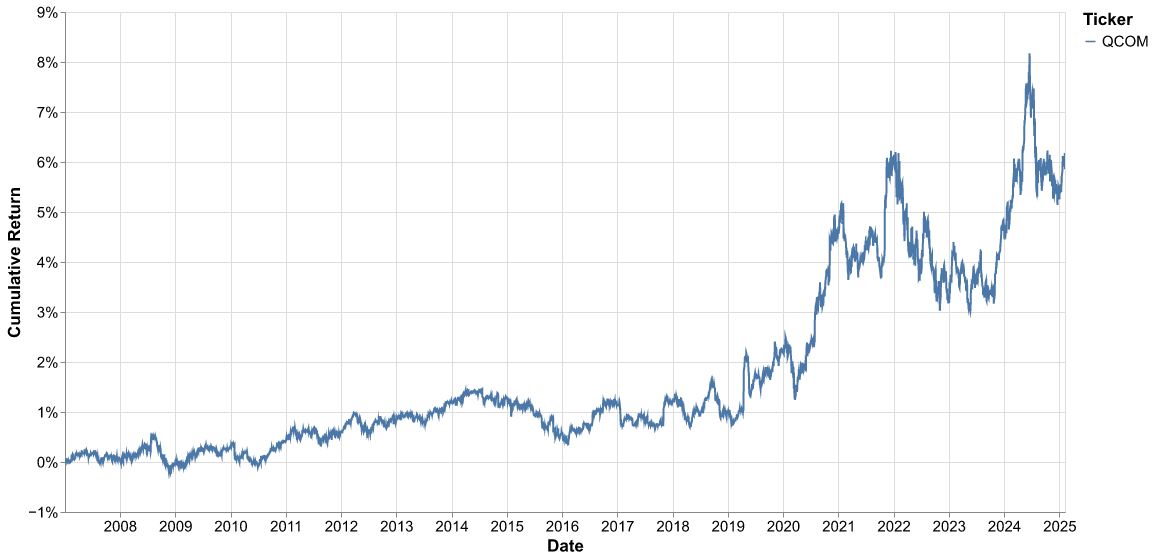
\includegraphics[width=0.9\linewidth]{content/plots/cumulative_returns_qcom}
	\caption{Cumulative Returns for the sample securities}
	\label{fig:cum_returns}
\end{figure}
Figure (\ref{fig:cum_returns}) shows the cumulative returns for QCOM. Cumulative returns ignore risk and measure the total percentage return, whereas metrics such as the standard deviation, $\hat{\sigma}_x$, and kurtosis, $\hat{K}(x)$, account for risk. The idea of studying volatility is that the returns of our asset $\lbrace r_t\rbrace$ have a serial correlation, or it may merely be stationary. The Autocorrelation Function (ACF) measures the correlation between a time series and its own past values at different lags. It helps identify patterns, dependencies, and stationarity in time series data. When considering a weakly stationary return series, $r_t$, the linear dependence between $r_t$ and past values of $t_{t-i}$ is called the lag-$\ell$ autocorrelation of $r_t$, denoted by the following:
\begin{equation}
	\hat{\rho}_\ell=\frac{\sum_{t=\ell+1}^{T}\left(r_t-\bar{r}\right)\left(r_{t-\ell}-\bar{r}\right)}{\sum_{t=1}^{T}\left(r_t-\bar{r}\right)^2},\quad 0\leq\ell<T-1
\end{equation}
For testing several autocorrelations jointly, we have the Ljung and Box test, denoted by,
\begin{equation}
	\mathcal{Q}(m)=T(T+2)\sum_{\ell=1}^{m}\frac{\hat{\rho}_\ell^2}{T-\ell}
\end{equation}
The hypothesis test for Ljung and Box is established as follows:
\[
\begin{aligned}
	H_0&:\rho_1=\cdots=\rho_m=0\\
	H_a&:\rho_i\neq 0
\end{aligned}
\]
for some $i\in\lbrace1,\ldots,m\rbrace$. We assume that $\lbrace r_t\rbrace$ is an iid sequence and $\mathcal{Q}^*(m)$ is a chi-squared random variable, $\mathcal{X}$, with $m$ degrees of freedom. The decision rule is to reject $H_0$ if $\mathcal{Q}(m)>\mathcal{X}^2_\alpha$, where $\mathcal{X}^2_\alpha$ denotes the $100\left(1-\alpha\right)$th percentile of a chi-squared distribution. 

Figure (\ref{fig:acf_plot}) shows the sample autocorrelation functions of the monthly log returns from January 2007 to November 2025. We have used a maximum of 20 lags. In each plot, two horizontal dashed lines denote two standard error limits of ACF. The sample ACFs or the MSFT plot are very close to each other, and they suggest that the serial correlations of monthly MSFT log stock returns are very small, if any. The sample ACFs are all within their two standard error limits, indicating that they are not significantly different from zero at the 5\% level.

\begin{figure}[h]
	\centering
	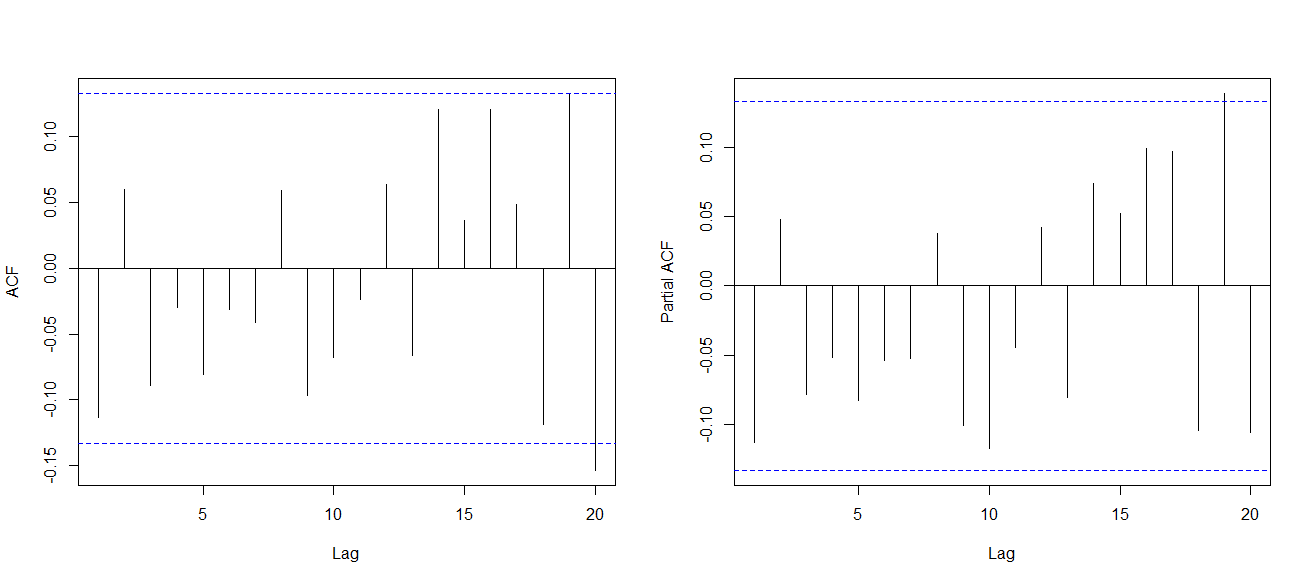
\includegraphics[width=0.9\linewidth]{content/plots/qcom_acf_pacf.png}
	\caption{ACF and PACF of QCOM}
	\label{fig:qcom_acf_pacf}
\end{figure}

Regarding the log monthly returns for the other securities in our sample, we find there is at least one lag that determines a significant serial correlation with previous returns. For QCOM, this occurs at lag 17, From looking at the ACF plots, it would appear that these lags barely reach the rejection threshold of 2 times the standard error. However, we can perform the Ljung-Box statistic determine if there are some significant serial correlations at the 5\% level for all return series. The Ljung-Box statistic with the max lag gives us a p-value of 0, so we reject the null-hypothesis.

As we can see from the test statistics and the $p$-values, the only securities with a significant serial correlation with monthly log returns are QCOM. What we can interpret from this data, at least for long monthly returns, is that there is no significant serial correlation. It may be worth using a more frequent observation series, such as daily.

We have also looked at the Partial Autocorrelation Function (PACF) of the log monthly returns. The PACF is used to directly measure the relationship between a time series and its past values at different lags while removing the influence of the intermediate lags. Unlike the ACF, which includes direct and indirect correlations, the PACF isolates the pure effect of each lag on the present value.

Figure (\ref{fig:pacf_plot})shows the PACF for the log monthly returns for our sample securities. We have used a maximum of 20 lags. After accounting for intermediate lags, each bar in the PACF plot represents the correlation between the time series and its lagged version. The dashed lines represent the 95\% confidence interval. Any bar extending beyond these lines is statistically significant. ADBE and CSCO all appear to have significant lags.

ADBE have significant lags at month 6 and month 12; meaning the returns 6 and 12 months have a direct influence on the current month returns. This suggest that monthly log returns of ADBE may have some seasonal dependency. With CSCO, we have significant lags at month 6 and 14, suggesting the log monthly returns from 6 and 14 months ago have a direct influence on the log monthly returns in the current month.
\section{Unit-root and Seasonality}
To test whether the log price $p_t$ of an asset follows a random walk, we would need to employ the following models
\begin{equation}
	\begin{aligned}
		p_t&=\phi_1p_{t-1}+\epsilon_t\\
		p_t&=\phi_0+\phi_1p_{t-1}+\epsilon_t
	\end{aligned}
\end{equation}
where $\epsilon_t$ denotes the error term. We need to consider the null hypothesis
\begin{equation}
	\begin{aligned}
		&H_0:\phi_1=1\\
		&H_a:\phi_1<1.
	\end{aligned}
\end{equation}
Where the test statistic is
\begin{equation}
	\hat{\phi}_1=\frac{\sum_{t=1}^{T}p_{t-1}p_t}{\sum_{t=1}^{T}p^{2}_{t-1}},\quad\hat{\sigma}^2_\epsilon=\frac{\sum_{t=1}^{T}(p_t-\hat{\phi}_1p_{t-1})^2}{T-1}
\end{equation}
where $p_0=0$ and $T$ is the sample size. If the null hypothesis shows that $\phi_1=1$, we fail to reject the null hypothesis, which say that the time series has a Unit Root. Otherwise, we can reject the null hypothesis and consider the time series as stationary. We perform this hypothesis test with a technique commonly referred to as the augmented Dickey-Fuller (ADF) unit-root test.

\begin{figure}[h]
	\centering
	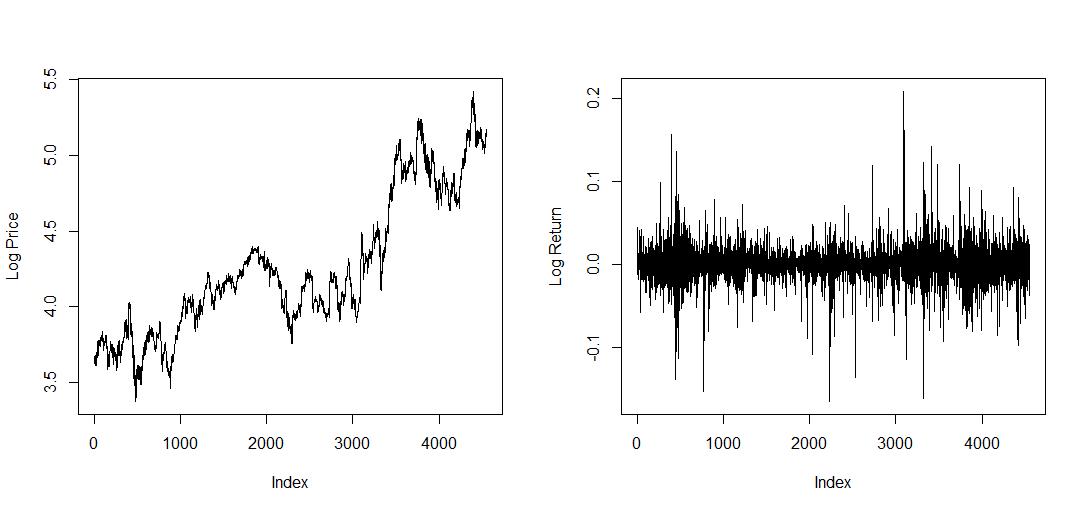
\includegraphics[width=0.9\linewidth]{content/plots/qcom_log_price_return.png}
	\caption{Time Series of QCOM Log Prices and Returns }
	\label{fig:qcom_log_price}
\end{figure}

Figure (\ref{fig:qcom_log_price}) shows the log returns and prices of the QCOM. We took the log transformation for two reasons. First, it is used to handle the exponential growth of the series, which the plot on the left confirms that the growth is linear on a log scale. Second, the transformation is used to stablize the variability of the series. With these adjustments in mind, we can see that the log price exhibit an upward trend. On the other hand, the variability changes throughout the time series when it comes to the log returns. Despite this, the log of the log returns is clearly stationary. We implemented the augmented Dickey-Fuller test on both the log prices and returns.
\begin{table}[ht]
	\centering
	\caption{Augmented Dick-Fuller Test for QCOM}
	\begin{tabular}[t]{lcccc}
		\toprule
		Time Series &Lag order& t-statistic & $p$-value & Outcome  \\
		\midrule
		Log Prices & 16 & -3.051 & 0.1333 & Unit-Root  \\				
		Log Returns & 16 & -16.254 & 0.01 & Stationary  \\				
		\bottomrule
	\end{tabular}\label{tab:adftest}
\end{table}
Table (\ref{tab:adftest}) shows the output of the augmented Dickey-Fuller test for the log prices and returns of QCOM. As we can see our suspicions were correct; we fail to reject the null-hypothesis for the log prices, but reject the null-hypothesis for the log returns. As such, the log returns are stationary, while the log prices exhibit unit-root.

We establish the time series' seasonality by examining the log prices' sample ACF. Figure (\ref{fig:qcom_acf_plots}) shows the ACF plots of QCOM with varying differencing and seasonality implementations. We have used a maximum lag of 100, with the time and seasonal differencing of once every 30 lags. The autocorrelation plot on the top right contains a very high and slow decay, starting from 1 at lag 0, which decreases gradually. This is typical of a non-stationary time series, where the values of the sample ACF are highly dependent on their past, such as a random walk.

\begin{figure}[h]
	\centering
	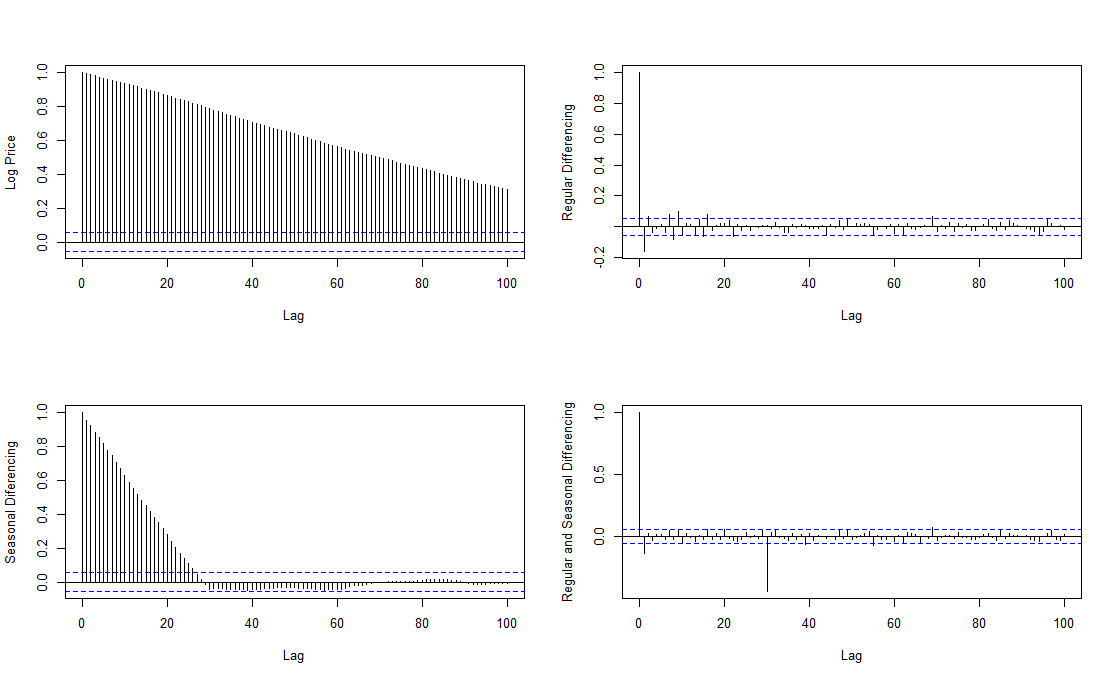
\includegraphics[width=1\linewidth]{content/plots/acf_plot_time_series.png}
	\caption{ACF Plot of QCOM }
	\label{fig:qcom_acf_plots}
\end{figure}

The plot on the top right shows the ACF of the First differenced log prices of the daily log prices. We can see a sharp drop in the autocorrelation at lag 1, where the other lags are within the confidence bounds. The first differencing has successfully removed the trend, producing a series that now looks more like white noise. 

On that bottom left plot, we have the ACF of the seasonal differencing, with a strong autocorrelation at lower lags, which slowly decreases to zero around lag 30. The differencing involves the following formula

\begin{equation}
	\Delta_{30}(\Delta x_t)=(1-B^{30})\Delta x_t=\Delta x_t-\Delta x_{t-30}
\end{equation}

After lag 30, the values fluctuate randomly around zero. This suggests that seasonal differencing alone removes the long-run periodicity but not the trend of the time series. In other words, seasonal differencing alone is not enough to transform the plot into a stationary time series.

The final plot on the bottom right shows the ACF after regular and seasonal differencing. The pattern shows that almost all autocorrelations are within the confidence bands, except for a substantial spike at lag one and lag 30, which suggest a seasonal lag. As we can see, combining regular and seasonal differencing yields a stationary series, and the residual autocorrelations are minimal. These transformations show that the plots on the bottom left and right show a stationary transformation. Fitting an ARIMA model would involve implementing either regular differencing or both regular and seasonal differencing.